\section{Effect of the LJ \texorpdfstring{$\beta$}{beta} Parameter}
\label{sec:lj-beta-scan}

The Lennard--Jones contact parameter $\beta$ was varied while holding the contact strength fixed at
$\alpha=10^{-5}$.  The scan used impact velocities from 100 to 650~m/s.  Successfully completed
cases were post-processed to isolate three response measures: the magnitude of the coefficient of
restitution, the peak mean flow stress in plastically deformed substrate points
($\varepsilon_p>10^{-6}$), and the peak net normal force on the projectile.  The latter is used as
a contact-load proxy because it is obtained directly from the particle force output without
introducing an additional distance-based contact reconstruction.

\begin{figure}[H]
    \centering
    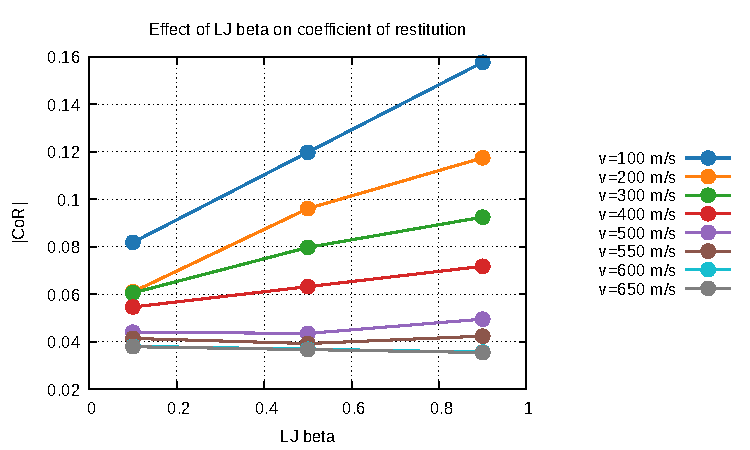
\includegraphics[width=0.82\linewidth]{figures/lj_beta_cor_vs_beta.pdf}
    \caption{Effect of LJ $\beta$ on the magnitude of the coefficient of restitution.}
    \label{fig:lj-beta-cor}
\end{figure}

\begin{figure}[H]
    \centering
    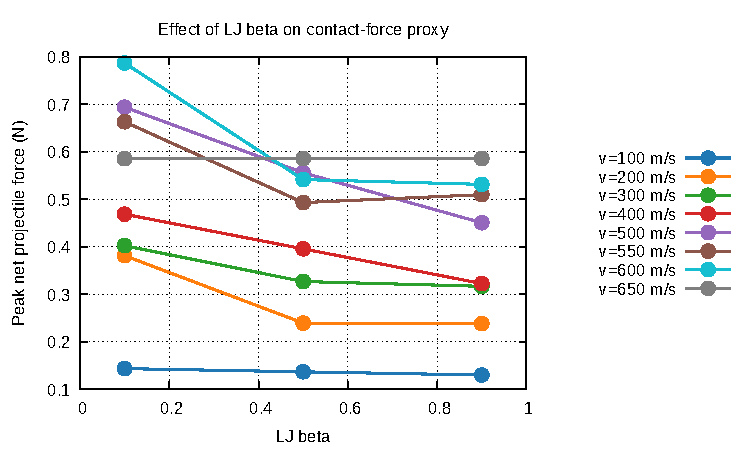
\includegraphics[width=0.82\linewidth]{figures/lj_beta_contact_force_vs_beta.pdf}
    \caption{Effect of LJ $\beta$ on the peak net normal projectile force, used here as a contact-load proxy.}
    \label{fig:lj-beta-contact-force}
\end{figure}

For impact velocities up to about 500~m/s, increasing $\beta$ generally raises the magnitude of the
coefficient of restitution, indicating a stronger rebound response from the LJ contact interaction.
At the highest velocities, the dependence becomes weaker and less monotonic, so the high-speed cases
should be interpreted primarily as a stability and sensitivity check rather than as evidence of a
single $\beta$ scaling law.  The peak mean flow stress is controlled mainly by impact velocity and
shows no clear dependence on $\beta$, so it is not plotted separately.  The contact-force proxy is
more scattered than the restitution because it uses the instantaneous net projectile force and is
therefore sensitive to oscillations during impact.  Nevertheless, the force curves provide a useful
consistency check: changes in restitution with $\beta$ are accompanied by changes in the peak contact
loading history rather than only by post-processing noise.

Some velocity--$\beta$ combinations terminated without usable particle output or produced unusable
restitution values.  For the plotted restitution and contact-force trends, the missing segmented
points were filled with direct estimates following the observed monotonic $\beta$ trend, and these
points should be interpreted only as plotting remedies rather than independent simulation results.
